\documentclass[11pt]{article}
\usepackage[a4paper, left=2cm, right=2cm, top=2.5cm, bottom=2.5cm]{geometry}
\usepackage{graphicx}
\usepackage{natbib}
\usepackage[toc,page]{appendix}
\usepackage{float}
\usepackage{amsmath}
\usepackage{varwidth}
\usepackage{xcolor}
\usepackage{url}
\usepackage[font=footnotesize]{caption}
\usepackage{subfig}
\usepackage{hyperref}

% Comment if need more space
\usepackage{setspace} \doublespacing\setlength{\jot}{10pt}

% Indentation for first paragraph
\usepackage{indentfirst}
\setlength{\parindent}{1.5em}

\newcommand{\grad}{\operatorname{grad}}
\newcommand{\dive}{\operatorname{div}}
\DeclareMathOperator{\g}{g}
\DeclareMathOperator{\G}{G}
\DeclareMathOperator{\T}{T}



\begin{document}

% Cover Page
\begin{titlepage}

    \begin{flushleft}
        
\includegraphics[width=8.5cm]{Images/centra.png}
    \end{flushleft}

    \begin{flushright}
        \vspace{-2.2cm}
        
\includegraphics[width=4cm]{Images/college_logo.jpg}
    \end{flushright}
    
    \vspace{7cm}
    
    \centering
    {\huge\textbf{Gravitational Collapse using Null Coordinates} \par}
    
    \vspace{5cm}
    
    {\large First Cycle Integrated Project in Engineering Physics\par}
    \vspace{3cm}
    {\large Joana Yao\par}
    \vspace{0.5cm}
    {\large Orientation: David Hilditch\par}
    
    \vfill
    
    {\large 2024\par}
\end{titlepage}

% Abstract
\noindent
\hrulefill% Upper horizontal line
\begin{center}
    \section*{Abstract}

\end{center}
\hrulefill% Lower horizontal line
\vspace{0.5cm}

\section{Introduction}

This project aims to make a programme to solve the Einstein-scalar Equations in null coordinates with spherical symmetry with initial conditions in a null slice and replicate the result in the paper \textcolor{red}{write reference}

and see if it collapses or not and blabla I probably cant even do this

The ones who worked in this are blabla and bla


\subsection{Formulation of null initial value problem}

In general, a spherically symmetric metric in null coordinates is
\begin{align}
    ds^2 = 2g_{uv}dudv + r^2d\Omega^2\, ,
\end{align}
where $u$ and $v$ are the null coordinates $d\Omega^2 = d\theta^2+\sin^2\phi\,d\phi^2$ is the metric for a 2-sphere, and $r$ is the usual radial coordinate, which will be regarded as a function of $u$ and $v$. The coordinates are defined as follows: $u$ is the proper time of an observer at the origin (that is, at r=0) and is constant on outgoing light rays and $u$ = 0 is the initial data surface; the coordinate $v$ is constant on ingoing light rays and is equal to the usual area coordinate $r$ on the initial data surface.

The Einstein Equations for a scalar field are given by
\begin{align}
    R_{\mu\nu}=8\pi\partial_\mu\Phi\partial_\nu\Phi 
    \label{eq: Einstein eqs}
\end{align}
where $R_{\mu\nu}$ is the Ricci tensor (related to the metric $g_{\mu\nu}$) and $\Phi$ is the scalar field. \textcolor{red}{Put def of ricci tensor, maybe on annex}

We now introduce the notation used from here on. For any function f, we define
\begin{gather}
    \Bar{f} \equiv \frac{1}{r}\int_0^r f dr = \frac{1}{r}\int_{r=0}^v f(u,\tilde{v}) r'(u,\tilde{v}) d\tilde{v}\, ,\label{eq: bar definition}\\
    f' \equiv \frac{\partial f}{\partial v} \, ,\\
    \dot f \equiv \frac{\partial f}{\partial u} \, .
\end{gather}
where the $r=0$ in the integral limit means $v$ such that $r(u,v)=0$ .

Now, defining $h$ such that $\bar h = \Phi$, we can use the Einstein equations to write the metric as a function of $h$ and $r$. We also define some useful quantities
\begin{gather}
    q \equiv r^{-1}(h-\bar h)^2 \, ,\\
    g \equiv \exp{(4\pi r \bar q)} \, .
\end{gather}
Then the $(\theta,\theta)$ equation in \eqref{eq: Einstein eqs} gives
\begin{align}
    1- 2\frac{\partial_v r\partial_u r + r \partial_u\partial_v r}{g_{uv}} = 0 \Leftrightarrow
    g_{uv} = 2 \partial_v (r \partial_u r) \Leftrightarrow 
    \frac{1}{2r}\int_{r=0}^v g_{uv}(u,\tilde{v}) d\tilde{v} = \dot r \, ,
\end{align}
and the $(v,v)$ equation yields
\begin{align}
    &\frac{2 \partial_v g_{uv}\partial_v r - 2g_{uv}\partial_v^2 r}{g_{uv}r} = 8\pi(\partial_v \bar h)^2 \\
    \Leftrightarrow
    &\frac{\partial_v g_{uv}}{g_{uv}} = \frac{4\pi r (\partial_v \bar h)^2 + \partial_v^2 r}{\partial_v r} \,\\
     \Leftrightarrow
    &\frac{g_{uv}}{g_{uv}(r=0)} = \exp{\left[\int_{r=0}^v \frac{4\pi r (\partial_v \bar h)^2}{\partial_v r} + \partial_v \ln{\partial_v r}\,d\tilde{v}\right]} .\label{eq: (v,v) equation}
\end{align}
Using some arithmetric and the definition in equation \eqref{eq: bar definition} we get
\begin{align}
    \partial_v \Bar{h} = \frac{r'}{r}(h-\Bar{h}) \, ,
\end{align}
so the equation \eqref{eq: (v,v) equation} becomes 
\begin{align}
    &g_{uv} = g_{uv}(r=0)\exp{(4\pi r \bar{q}) + \ln{(r')} - \ln{(r'(r=0))}}\\
    &g_{uv}= - r'g
\end{align}
where in the last step we used $g_{uv}(r=0) = -1$ (which comes from the definition of the null coordinates)\textcolor{red}{explain why} and we choose $r'(r=0) = 1$ (which is just a matter of a scale factor).

\section{Simpson Rule}

In this project, we used Simpson's rule for irregularly spaced data to integrate. In this method, the integral in an interval $[a,b]$ with an even number $N$ of sub-intervals $h_k$ is given by
\begin{align}
    \int_a^b f(x) dx\approx\sum_{i=0}^{N/2-1}\frac{h_{2i}+h_{2i+1}}{6}\left[\left(2-\frac{h_{2i+1}}{h_{2i}}\right)f_{2i}+\frac{(h_{2i}+h_{2i+1})^2}{h_{2i}h_{2i+1}}f_{2i+1}+\left(2-\frac{h_{2i}}{h_{2i+1}}\right)f_{2i+2}\right] \, .
    \label{eq: simpson rule}
\end{align}

In the case the number of slices $N$ is odd, we use the formula \eqref{eq: simpson rule} up until the second to last interval and then add the quantity
\begin{align}
    &\alpha f_N + \beta f_{N-1} - \eta f_{N-2}\, ,
\end{align}
where
\begin{align}
    &\alpha=\frac{2h_{N-1}^2+3h_{N-1}h_{N-2}}{6(h_{N-2}+h_{N-1})}\, ,\\
    &\beta=\frac{h_{N-1}^2+3h_{N-1}h_{N-2}}{6h_{N-2}}\, ,\\
    &\eta=\frac{h_{N-1}^3}{6h_{N-2}(h_{N-2}+h_{N-1})}\, .
\end{align}


\subsection{Method Order}

\subsection{Convergence}

To test this algorithm, we used as integrand a Gaussian distribution with $\sigma=1$ and $\mu=0$, integrating it between -5 and 5, resulting in the figure \ref{fig:gauss_integral}. We can see the result looks reasonably satisfactory.

\begin{figure}[H]
    \centering
    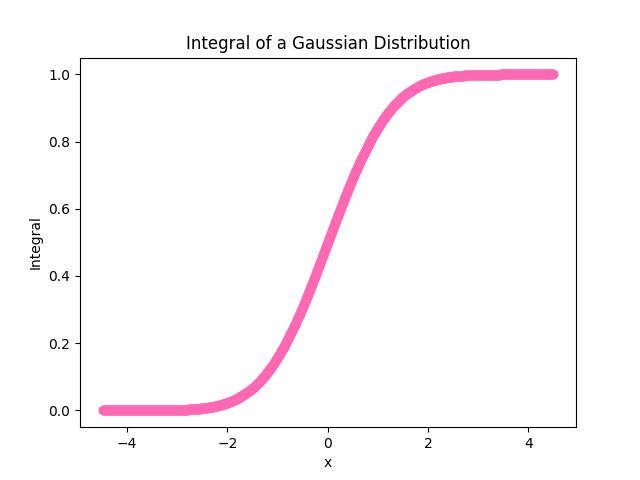
\includegraphics[width=0.5\linewidth]{Images/gauss_integral.png}
    \caption{Integral of a Gaussian distribution with $\sigma=1$ and $\mu=0$ using the Simpson Rule}
    \label{fig:gauss_integral}
\end{figure}

To conclude the result is indeed satisfactory, we check the convergence of the Simpson Rule. For that, we need to differentiate the points where the integral is calculated with an even number of slices or with an odd number of slices because the method is different for each of them.


\begin{figure}[H]
    \centering
    \subfloat[Odd slices]{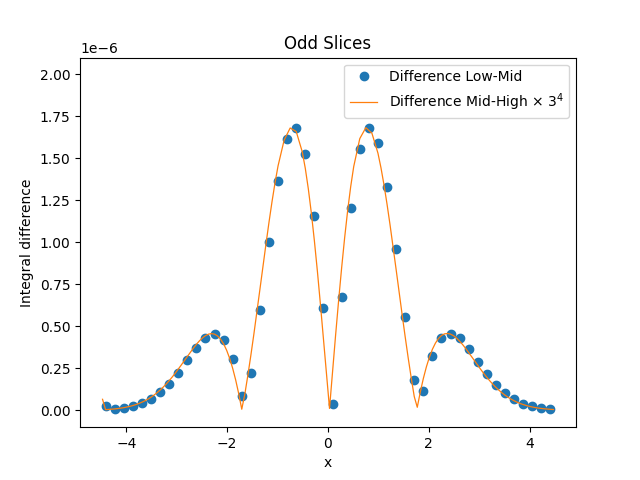
\includegraphics[width= 0.5\linewidth]{Images/Simp_convergence_odd.png}}
    \subfloat[Even slices]{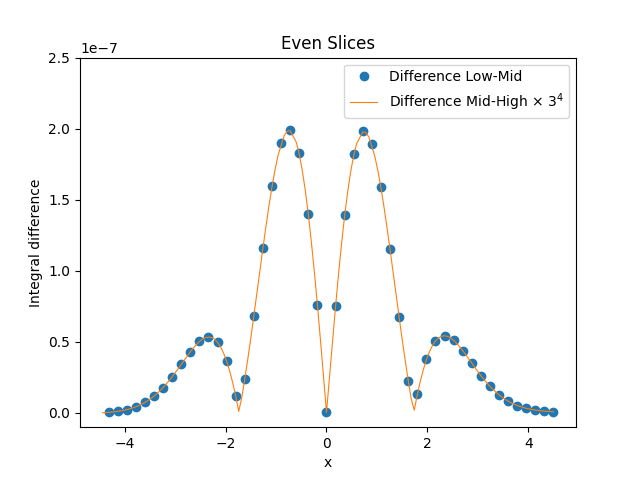
\includegraphics[width= 0.5\linewidth]{Images/Simp_convergence_even.png}}
    \caption{Comparison of the difference between the obtained integral with low (step = 0.09) and middle (step = 0.3) resolution, and of the different between the obtained integral with middle (step = 0.03) and high (step = 0.1), where the later one is multiplied by $3^4$. }
    \label{fig:simp_conv}
\end{figure}




\section{Runge-Kutta}

\section{Fit to the origin}

\section{GR equations}

\section{Applying to GR}

\section{Conclusions}

% Appendix
\appendix

% References

\bibliographystyle{unsrt} % Set bibliography style
\bibliography{references.bib}


%\end{multicols}

\end{document}
